\chapter{Fundamentals}
 In this chapter, we first review some fundamental properties of continuous dynamical systems that will be used heavily in later chapters. As we will see, these technical results are interesting in their own right. They can help in interpreting or cross-checking numerical results or physical models for self-consistency or accuracy.
\section{Existence and uniqueness of solutions}
Consider  
\begin{align}
\begin{dcases}
	\dot{ {x}} = f( {x},t); &  {x} \in \mathbb{R}^{n} \\
	 {x}(t_0) =  {x}_0
\end{dcases}.
\end{align}
Does this initial value problem have a unique solution? We have the following theorems to help us answer that question.
\begin{theorem}[Peano]
	\label{thm:Peano}
	If $f\in C^0$ near $( {x}_0, t_0)$, then there exists a local solution $\varphi(t)$, i.e., 
\begin{align}
	\dot{\varphi}(t) = f(\varphi(t), t), \varphi(t_0) = x_0;\ \forall  t\in (t_0 - \epsilon, t_0 + \epsilon);\ 0<  \epsilon \ll 1.
\end{align}
\end{theorem}
\begin{ex}[Free falling mass]
	Consider a point mass of mass $m$ at position $x$. The acceleration due to gravity is denoted by $g$. Measuring the potential energy from the reference point $x=x_0$, we have the total energy is conserved.
	\begin{align}
		\frac{1}{2} m \dot{x}^2 = mg(x-x_0).
	\end{align}
This implies that
\begin{align}
	\begin{dcases}
		\dot{x} = \sqrt{2g(x-x_0)} \\
		x(0) = x_0
	\end{dcases}
\end{align}
on the set $P = \{ x \in \mathbb{R}:\ x \geq x_0\}$. Therefore we have that $f\in C^0$ in phase space, so by Peano's theorem (cf. Theorem \ref{thm:Peano}), there exists a local solution. A schematic diagram is shown in Fig. \ref{fig:point_mass}. 
	\begin{figure}[h!]
		\centering
		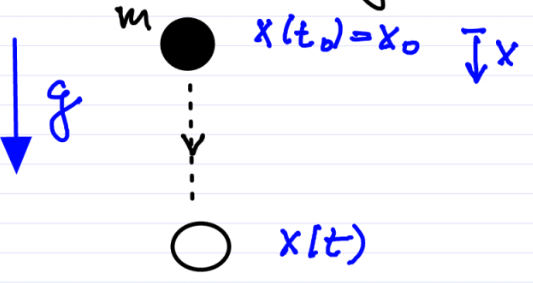
\includegraphics[width=0.4\textwidth]{figures/ch1/1freefall.png}
		\caption{Schematic diagram of the point mass in free fall.}
		\label{fig:point_mass}
	\end{figure}
	The solution is actually $x(t) = x_0 + \frac{g}{2}(t-t_0)^2$, however $x(t) = x_0$ is also a solution to the IVP, therefore we do not have a unique solution. Physically there exists a solution, but this IVP was derived from a heuristic energy-principle, not from Newton's laws, which are not equivalent.
\end{ex}
\begin{definition}
A function $f$ is called locally Lipschitz around $ {x}_0$ if there exists an open set $U_{ {x}_0}$ and $L>0$ such that for all $ {x}, {y} \in U_{ {x}_0}$
\begin{align}
	\boxed{\left \| f( {y},t) - f( {x},t)\right \| \leq L  \| {y} -  {x} \|.}
\end{align}
\end{definition}

\begin{ex}[Lipschitz functions]
	Fig. \ref{fig:Lipschitz_ex} shows an example of a Lipschitz and a non-Lipschitz function around $x_0$.
	\begin{figure}[h!]
		\centering
		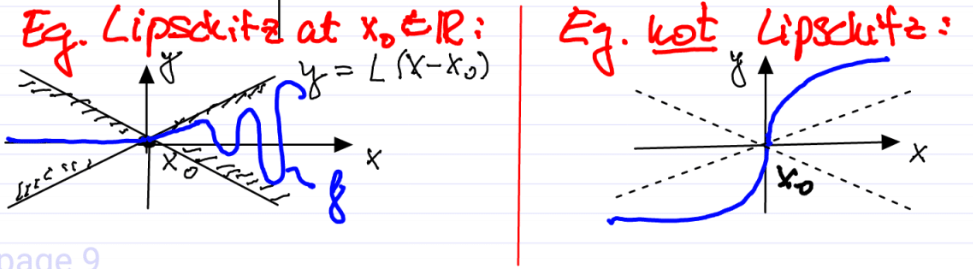
\includegraphics[width=0.8\textwidth]{figures/ch1/2lipschitz.png}
		\caption{Interpretation of the Lipschitz property.}
		\label{fig:Lipschitz_ex}
	\end{figure}
\end{ex}

\begin{theorem}[Picard]
	Assume 
	\begin{enumerate}
		\item  $f \in C^0$ in $t$ near $(t_0,  {x}_0)$,
		\item $f$ is locally Lipschitz in $ {x}$ near $(t_0,  {x}_0)$.
	\end{enumerate}
	Then there exists a unique local solution to the IVP. The proof can be found in Arnold's book on ODEs. 	
\end{theorem}
\textbf{Note} the following relations. If $f$ is $C^1$ $\implies$ $f $ is Lipschitz $\implies $ $f$ is $C^0$.
\begin{ex}[Free falling mass revisted]
	We check if $f$ is Lipschitz.
	\begin{align}
		\frac{ \| f(x) - f(x_0)  \|}{ \|x-x_0 \|} = \frac{\sqrt{2g}}{\sqrt{ \|x-x_0 \|}} \geq  L  \| x - x_0 \|.
	\end{align}
Thus $f$ is not Lipschitz near $x_0$.	
\end{ex}

\section{Geometric consequences of uniqueness}
If the solution is unique, we have a few facts that can be derived from the geometric point of view.
\begin{enumerate}
	\item The trajectories of autonomous systems cannot intersect. Note that fixed points do not violate this (e.g. pendulum equations). See Fig. \ref{fig:pend_phase_portrait} which shows the phase portrait of the pendulum.
		\begin{figure}[h!]
			\centering
			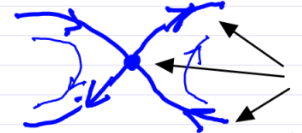
\includegraphics[width=0.3\textwidth]{figures/ch1/3pendulum_trajectories.png}
			\caption{The phase portrait of the pendulum. Trajectories do not intersect since each arrow is pointing at separate trajectories.}
			\label{fig:pend_phase_portrait}
		\end{figure}
		
	\item For non-autonomous systems, intersections in phase space are possible: a trajectory may occupy the same point $x$ at a different time instants (see the left panel of Fig. \ref{fig:automization}. In this case we can extend the phase space in order to get an autonomous system where there cannot be any intersections.
		\begin{figure}[h!]
			\centering
			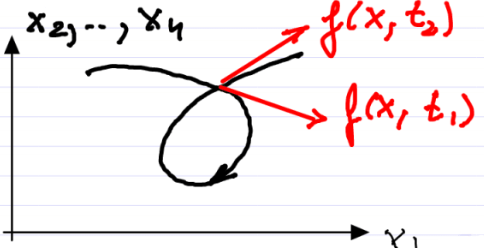
\includegraphics[width=0.4\textwidth]{figures/ch1/4intersecting_trajectories.png}
			\hspace{0.05\textwidth}
			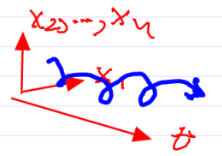
\includegraphics[width=0.3\textwidth]{figures/ch1/5extended_space.png}
			\caption{Left: Intersecting trajectories in phase space for a non-autonomous system. Right: The same trajectory in the extended phase space, without intersections.}
			\label{fig:automization}
		\end{figure}
		\begin{align}
			 {X} = 
			\begin{pmatrix}
				 {x} \\ t
			\end{pmatrix},\
			F( {X}) = 
			\begin{pmatrix}
				f( {x},t) \\ 1
			\end{pmatrix};\
			\dot{ {X}} = F( {X}).
		\end{align}
\end{enumerate}

\section{Local vs global existence}
\begin{ex}[Exploding solution]
	\begin{align}
		\begin{dcases}
			\dot{x} = x^2 \\
			x(t_0) = 1.
		\end{dcases}
	\end{align}
	Integrating yields the solution $x(t) = \frac{1}{1 - (t-t_0)}$. This solution blows up at $t_{\infty }=t_0 + 1$, therefore the solution is only local. This is demonstrated in Fig. \ref{fig:exploding_solution}.	
\begin{figure}[h!]
\centering	
\begin{tikzpicture}
	\begin{axis}
		[xmin=0, xmax=2.5, ymin=0.5, ymax=3, domain = 1:1.9, xlabel=$t$, ylabel=$x(t)$, xtick=\empty, ytick=\empty]
		\addplot[color=black] {1/(2-x)};
		\addplot[color=black, dashed] coordinates {(1.7,0.5) (1.7,3.1)} node[pos=0, above right] {$t_{\infty }$};
		\addplot[color=black, dashed] coordinates {(1,0.5) (1,1)} node[pos=0, above right] {$t_{0}$};
		\addplot[color=black, dashed] coordinates {(0,1) (1,1)} node[pos=0, above right] {$x_{0}$};
	\end{axis}
\end{tikzpicture}
\caption{Solution to the ODE $\dot{x}=x^2$ started from $x(t_0)=1$.}
	\label{fig:exploding_solution}
\end{figure}
\end{ex}
To address this problem of local solutions not being able to be continued into global solution, we have the following theorem.
\begin{theorem}[Continuation of solution]
	If a local solutions cannot be continued to a time $t=T$, then we must have
	\begin{align}
		\boxed{\lim_{t\to T}  \| {x}(t) \|= \infty.}
	\end{align}
The proof can be found in Arnold's book on ODEs.	
\end{theorem}

\begin{ex}[Coupled Pendulum System]
	Consider two pendula of masses $m_1$ and $m_2$. They both have length $l$. The angles of these pendula are denoted by $\varphi_1$ and $\varphi_2$. Let us assume that they are coupled by a nonlinear spring, which can be described by a potential $V(\varphi_1, \varphi_2)$. This setup is illustrated in Fig. \ref{fig:coupled_pendulum}. We set $x_1 = \varphi_1,\ x_2 = \dot{\varphi_1},\ x_3 = \varphi_2,\ x_4=\dot{\varphi_2} $ and get the following equation of motion
\begin{align}
	\begin{dcases}
		\dot{x}_1 = x_2 \\ \dot{x}_2 = \ldots \\ \dot{x}_3 = x_4 \\ \dot{x}_4 = \ldots
	\end{dcases}
\end{align}
The RHS is smooth, therefore there exists a unique local solution to any IVP.
\begin{figure}[h!]
	\centering
	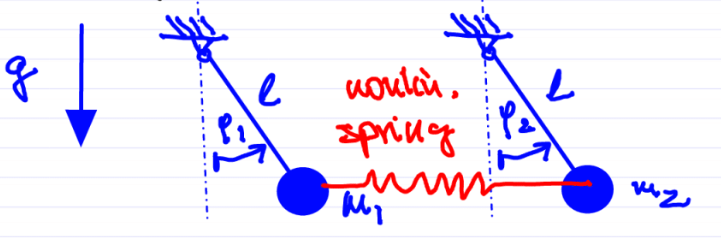
\includegraphics[width=0.6\textwidth]{figures/ch1/6coupled_pendulum.png}
	\caption{Physical setup of the coupled pendulum with a nonlinear spring.}
	\label{fig:coupled_pendulum}
\end{figure}
The phase space is given by 
\begin{align}
	P = \{ {x}:\ x_1 \in S^1,\ x_2 \in \mathbb{R},\ x_3 \in S^1,\ x_4 \in \mathbb{R} \} = S^1 \times \mathbb{R}\times S^1 \times \mathbb{R}.
\end{align}
Where $S^1$ is the 1 dimensional sphere (i.e. a circle). With this space we know that $ \|x_1 \|$ and $ \|x_3 \|$ are bounded. Due to energy being conserved we have
\begin{align}
	E &= T+V = \frac{1}{2}m_1 l_1 x_2^2 + \frac{1}{2}m_2 l_2 x_4^2 + \underbrace{V(x_1, x_3)}_{\geq 0}\\
	E &= E_0 =  \textrm{constant} \geq 0.
\end{align}
Hence $ \|x_2 \|$ and $ \|x_4 \|$ are also bounded, therefore all solutions exist globally.
\end{ex}
\begin{definition}
	A linear system is one such that for $ {x}\in \mathbb{R}^{n},\ {A}(t) \in \mathbb{R}^{n\times n}$ and ${A}\in C^0$ 
	\begin{align}
		\boxed{\dot{ {x}} = {A}(t)  {x}.}
	\end{align}
\end{definition}

\begin{remark}[]
	Note that ${A} $ can be written as ${A}={S} +{\Omega }$ where ${S} = \frac{1}{2}({A} + {A}^T)$ is symmetric (i.e. ${S} = {S}^T)$ and ${\Omega} = \frac{1}{2}({A} - {A}^T)$ is skew symmetric (i.e. ${\Omega} = -{\Omega}^T$). Furthermore the eigenvalues of ${S}$, $\lambda_i$, are all real and their respective eigenvectors, $e_i$, are orthogonal.
\end{remark}

\begin{ex}[Global existence in linear systems]
\begin{align}
	\langle  {x}, \dot{ {x}} \rangle &= \frac{1}{2} \frac{d}{dt}  \| {x}(t) \|^2 = \langle  {x}, {A}(t)  {x}\rangle = \langle  {x}, ({S}(t) + {\Omega}(t) )  {x} \rangle \\
				   &= \langle  {x}, S(t)  {x} \rangle + \underbrace{\langle  {x}, {\Omega}(t)  {x} \rangle}_{=0} \stackrel{(*)}{=} 
				   \sum_{i=1}^{n} \lambda_i(t) x_i^2 \\
				   &\leq \lambda_{ \textrm{max} }(t) \sum_{i=1}^{n} x_i^2 = \lambda _{ \textrm{max} }(t)  \|  {x}(t) \|^2.
\end{align}
Where in $(*)$ we used that $ {x} = \sum_{i=1}^{n} x_i  {e}_i $ with $ \| {e}_i \|=1$ and $ {e}_i \perp  {e}_j$ for all $i \neq j$. Thus we get
\begin{align}
	\frac{\frac{1}{2}\frac{d}{dt} \| {x}(t) \|^2}{ \| {x}(t) \|^2} \leq \lambda_{ \textrm{max} }(t) 
	\implies \int_{t_0}^{t} \log \left( \frac{ \| {x}(s) \|^2}{ \| {x}(t_0) \|^2} \right) ds \leq \lambda _{ \textrm{max} }(s) ds.
\end{align}
By exponentiating both sides, we obtain
\begin{align}
\boxed{  \| {x}(t) \| \leq  \| {x}(t_0)  \| \exp\left(\int_{t_0}^{t} \lambda_{ \textrm{max} }(s)ds\right).}
\end{align}
Therefore, by the continuation theorem, global solutions exist as long as $\int_{t_0}^{t} \lambda_{ \textrm{max} }(s) ds < \infty $.
\end{ex}

\section{Dependence on initial conditions}
Given the IVP
\begin{align}
	\begin{dcases}
	\dot{ {x}} = f( {x},t) \\  {x}(t_0) =  {x}_0.
	\end{dcases}
\end{align}
With $ {x} \in \mathbb{R}^{n}$ and $f\in C^r$ for some $r\geq 1$, we have the solution $ {x}(t; t_0,  {x}_0)$.

The dependence of the solution on initial data is of interest to us. This is due to us wanting the solution to be robust with respect to errors and uncertainties in the initial data. To address this, we have Theorem \ref{thm:robust_initial_conditions}.
\begin{theorem}[]
	If $f \in C^r$ for $r\geq 1$ then $ {x}(t; t_0,  {x}_0)$ is $C^r$ in $(t_0,  {x}_0)$. Proof in Arnold's ODE.
	\label{thm:robust_initial_conditions}
\end{theorem}

The geometric meaning of this is that for $U \subset P \subset \mathbb{R}^{n}$ we have that $F_{t_0}^{t}(U)$ is a smooth deformation of $U$ (cf. Fig. \ref{fig:deformation}).
\begin{figure}[h!]
	\centering
	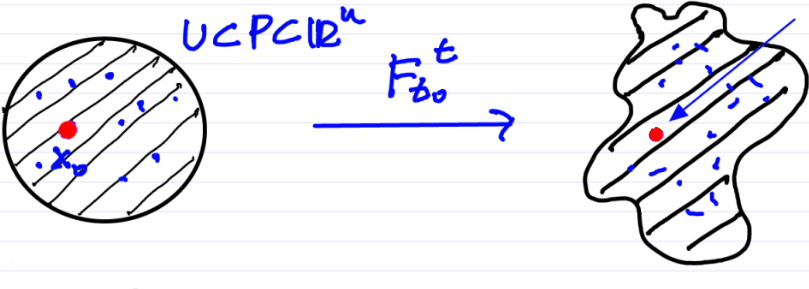
\includegraphics[width=0.7\textwidth]{figures/ch1/7smooth_transform.png}
	\caption{The smooth transformation of $U$. The red point on the right it $F _{t_0}^t( {x}_0)$, i.e. the image of $ {x}_0$ under the evolution operator.}
	\label{fig:deformation}
\end{figure}
It turns out $\left(F_{t_0}^{t}\right)^{-1} = F_{t}^{t_0}$ is also $C^r$, hence we have that $F_{t_0}^{t}$ is a diffeomorphism. 

Now, how can we compute the Jacobian of the flow map $\frac{\partial  {x}(t; t_0,  {x}_0)}{ \partial  {x}_0} = DF _{t_0}^{t}( {x}_0)$? We start from the IVP and take the gradient (with respect to $x_0$) of both sides. On the left hand side we can exchange order of the time derivative and the gradient and on the right hand side we use the chain rule. We end up with the equation
\begin{align}
	\frac{d}{dt}\frac{\partial  {x}}{\partial  {x}_0} = D_ {x} f( {x}(t; t_0,  {x}_0), t) \frac{\partial  {x}}{\partial  {x}_0}; \quad \frac{\partial x}{\partial x_0} \in \mathbb{R}^{n \times n}.
\end{align}
This means, that the flow map gradient satisfies the IVP
\begin{align}
	\frac{d}{dt}\left[ DF_{t_0}^{t}( {x}_0)\right] &= D_{ {x}}f(F_{t_0}^{t}( {x}_0), t) DF_{t_0}^{t}( {x}_0) \\
	DF_{t_0}^{t_0}( {x}_0) &= I.
\end{align}
This is called the equation of variations, which is a linear, non-autonomous ODE for the matrix $M = DF_{t_0}^{t}(x_0)$
\begin{align}
	\begin{dcases}
		\dot{M} = D_ {x} f( {x}(t; t_0,  {x}_0)) M \\ M(t_0) = I.
	\end{dcases}
\end{align}

\begin{ex}[Locations of extreme deformation in phase space]
	We define 
	\begin{align}
		 {\xi}(t) &:= \tilde{ {x}}(t) -  {x}(t) =  {x}(t; t_0, \tilde{ {x}}_0) -  {x}(t; t_0,  {x}_0)\\
		       &=  {x}(t; t_0,  {x}_0) + \frac{\partial  {x}}{\partial  {x}_0}(t; t_0,  {x}_0) {\xi}_0 + \mathcal{O}( \| {\xi}_0 \|^2) -  {x}(t; t_0,  {x}_0) \\
		       &= DF_{t_0}^{t}( {x}_0) {\xi}_0 + \mathcal{O}( \| {\xi}_0 \|^2).
	\end{align}
	Where we used the Taylor expansion and assume the perturbation to $ {x}_0$ is small, i.e. $ \| {\xi}_0 \| \ll 1$.
	\begin{figure}[h!]
		\centering
		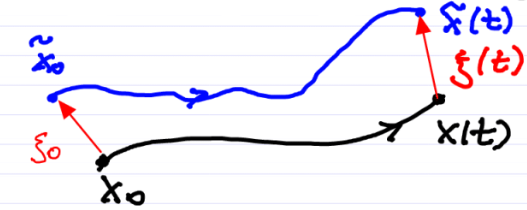
\includegraphics[width=0.5\textwidth]{figures/ch1/8dispersion.png}
	\end{figure}
	Therefore we have
	\begin{align}
		 \| {\xi}(t) \|^2 &= \langle DF_{t_0}^{t}( {x}_0)  {\xi}_0, DF_{t_0}^{t}( {x}_0) {\xi}_0 \rangle + \mathcal{O}( \| {\xi}_0 \|^3) \\
			   &= \langle  {\xi}_0, \underbrace{\left[ DF_{t_0}^{t}( {x}_0) \right]^T DF_{t_0}^{t}( {x}_0)}_{=: C_{t_0}^{t}( {x}_0)}  {\xi}_0 \rangle + \mathcal{O}( \| {\xi}_0 \|^3).
	\end{align}
	$C_{t_0}^{t}( {x}_0)$ is known as the Cauchy-Green strain tensor (field of $n\times n$ symmetric matrices).
	Therefore the largest possible deformation is
	\begin{align}
		\max_{ {x}_0, {\xi}_0} \frac{ \| {\xi}(t) \|^2}{ \| {\xi}_0 \|^2} = \max_{ {x}_0,  {\xi}_0}\frac{\langle  {\xi}_0, C_{t_0}^{t}( {x}_0)  {\xi}_0 \rangle}{ \| {\xi}_0 \|^2} = \max_{ {x}_0} \lambda_{n}( {x}_0).
	\end{align}
	Where we used that $C_{t_0}^{t}$ is positive definite in the last equality, and that $\lambda_n( {x}_0)$ is the largest eigenvalue of $C_{t_0}^{t}( {x}_0)$. Because we typically have exponential growth we introduce the following quantity.	
\end{ex}
\begin{definition}
	The finite-time Lyapunov exponent is defined as
	\begin{align}
		\boxed{ \textrm{FTLE} _{t_0}^{t}( {x}_0) := \frac{1}{2(t-t_0)} \log(\lambda_n( {x}_0)).}
	\end{align}
\end{definition}
The FTLE is a diagnostic quantity for Lagrangian Coherent Structures (LCS), i.e. influential surfaces governing the evolution in $P$.
\begin{figure}[h!]
	\centering
	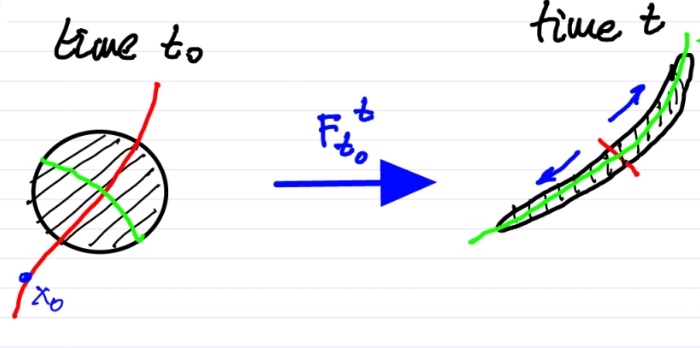
\includegraphics[width=0.6\textwidth]{figures/ch1/9deformation.png}
	\caption{On the left the red ridge represents large values of $ \textrm{FTLE} _{t_0}^{t}$, on the right the green ridge the high values of $ \textrm{FTLE} _{t}^{t_0}$.}
	\label{fig:FTLE_ridges}
\end{figure}
\begin{figure}[h!]
	\centering
	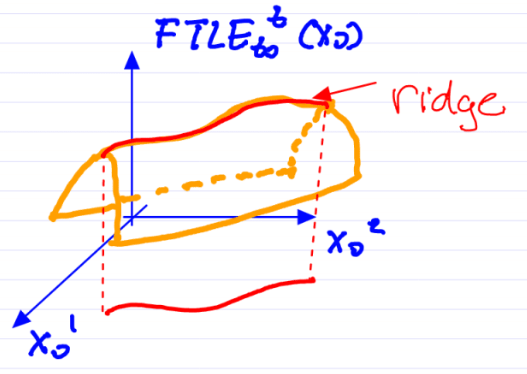
\includegraphics[width=0.4\textwidth]{figures/ch1/10ridge_projection}
	\caption{The projection of the FTLE ridge onto the initial value space.}
	\label{fig:FTLE_surface}
\end{figure}

The ridges of $ \textrm{FTLE} _{t_0}^{t}$ are the repelling LCS, meanwhile the ridges of $ \textrm{FTLE} _{t}^{t_0}$ are the attracting LCS as depicted in Fig. \ref{fig:FTLE_ridges}. Now we are left with the problem of computing $F_{t_0}^{t}( {x}_0)$. Recall that analytically we start with $F_{t_0}^{t}( {x}_0)$ and use this to calculate $DF_{t_0}^{t}( {x}_0)$. From here we can find $C_{t_0}^{t}( {x}_0)$, giving us $\lambda_n( {x}_0)$ and thereby the FTLE. We now outline a process to compute the FTLE numerically.
\begin{enumerate}
	\item Define an initial $M\times N$ grid of initial data $ {x}_0(i,j) \in \mathbb{R}^2$.
	\item Launch trajectories numerically from grid points to obtain a discrete approximation of $F_{t_0}^{t}( {x}_0)$ as $F_{t_0}^{t}( {x}_0(i,j))$.
	\item Use finite differencing to approximate 
		\begin{align}
			DF_{t_0}^{t}( {x}_0(i,j)) \approx
		\begin{pmatrix}
			\frac{x(t; t_0, x_0(i,j) + \delta e_1)_1 - x(t; t_0, x_{0}(i,j) - \delta e_1)_1}{2\delta} &
			\ldots &
			\frac{x(t; t_0, x_0(i,j) + \delta e_n)_1 - x(t; t_0, x_{0}(i,j) - \delta e_n)_1}{2\delta}\\
			\vdots & & \vdots \\
			\frac{x(t; t_0, x_0(i,j) + \delta e_1)_n - x(t; t_0, x_{0}(i,j) - \delta e_1)_n}{2\delta} &
			\ldots &
			\frac{x(t; t_0, x_0(i,j) + \delta e_n)_n - x(t; t_0, x_{0}(i,j) - \delta e_n)_n}{2\delta} 
		\end{pmatrix}
		.
		\end{align}
		
\end{enumerate}
This process then yields the surface we see in Fig. \ref{fig:FTLE_surface}.
\begin{ex}[Calculating the FTLE for the double gyre]
	Due to incompressibility, we can define the two dimensional flow using a single scalar function called the stream function.
\begin{align}
	\Psi(x,y) = -\sin(\pi x) \sin(\pi y).
\end{align}
	The components $(u,v)$ of the fluid velocity (${v} = (u,v)$) are obtained as partial derivatives of the stream function, according to the formulas
	\begin{align}
		\begin{dcases}
			u = \frac{\partial \Psi}{\partial y} \\ 
			v = \ - \frac{\partial \Psi}{\partial x}.
		\end{dcases}
	\end{align}
The Lagrangian trajectories of fluid particles obey the differential equations (i.e. we have the fluid velocity field)
\begin{align} 
	\begin{dcases}
		\dot{x} = u =  \frac{\partial \Psi}{\partial y} \\
		\dot{y} = v = - \frac{\partial \Psi}{\partial x}.
	\end{dcases}
\end{align}
Interestingly, in this case, the phase space coincides with the physical space spanned by the coordinates $(x,y)$.
\begin{remark}[]
	This is an example of a Hamiltonian system, where $\Psi$ is the Hamiltonian (usually denoted as $H$).
\end{remark}
For any autonomous Hamiltonian system we have that the Hamiltonian is constant along trajectories. We can verify this as follows
\begin{align}
	\frac{d}{dt}\Psi(x(t),y(t)) = \frac{\partial \Psi}{\partial x}\dot{x} + \frac{\partial \Psi}{\partial y}\dot{y} = 0.
\end{align}
So we have that trajectories are level curves of $\Psi(x,y)$. We can then derive the phase portrait from the level curves of $\Psi$. Further, we have that $\dot{x} = \frac{\partial \Psi}{\partial y} = - \pi \sin(\pi x) \cos(\pi y)$ which yields that $ \textrm{sign} (\dot{x}) = -  \textrm{sign} (\sin(\pi x))  \textrm{sign} (\cos(\pi y))$. Putting these together we can construct the contour plot with arrows. The contour plot, and FTLE approximation are shown in Fig. \ref{fig:FTLE_double_gyre}.

\begin{figure}[h!]
	\centering
	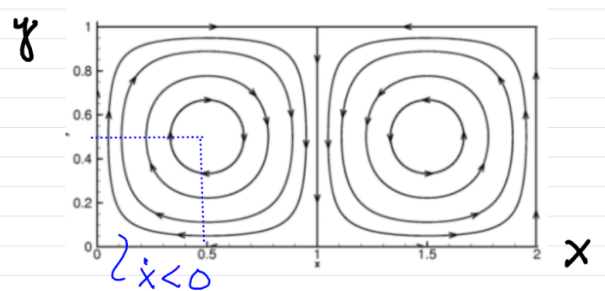
\includegraphics[width=0.5\textwidth]{figures/ch1/11contour_phase.png}
	\hspace{0.03\textwidth}
	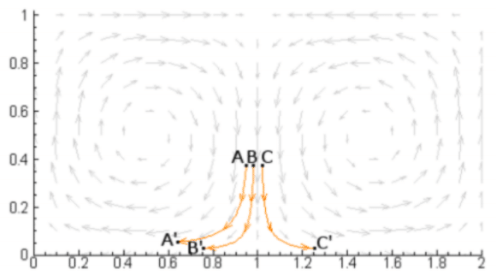
\includegraphics[width=0.45\textwidth]{figures/ch1/12ftle_exploration.png}
	\caption{}
	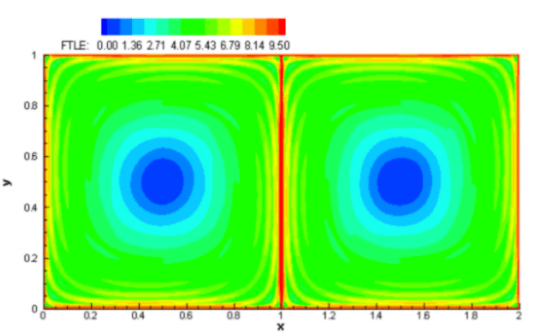
\includegraphics[width=0.5\textwidth]{figures/ch1/13ftle_final.png}
	\caption{Top left: The analytic phase plot. Top right: The exploration done to calculate FTLE. Bottom: The FTLE plot. Figures here were taken from Shawn Shadden of UC Berkeley.} \label{fig:FTLE_double_gyre}
\end{figure}
\end{ex}

\begin{ex}[ABC flow]
	Let our dynamical system be defined as follows with $A,B,C \in \mathbb{R}$
\begin{align}
	\begin{dcases}
		\dot{x} = A \sin(z) + C \cos(y) \\
		\dot{y} = B \sin(x) + A \cos(z) \\
		\dot{z} = C \sin(y) + B \cos(x).
	\end{dcases}
\end{align}
This is an exact solution to Euler's equations.  We have an autonomous velocity field. Depending on parameters it can even generate chaotic fluid trajectories. The numerical approximation of the FTLE for the ABC flow is depicted in Fig. \ref{fig:FTLE_flows}.
\begin{figure}[h!]
	\centering
	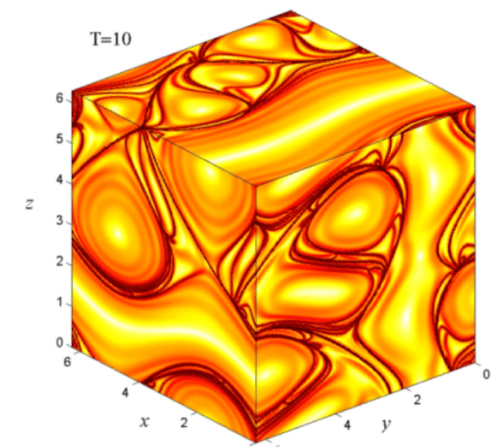
\includegraphics[width=0.4\textwidth]{figures/ch1/14fluid1.png}
	\hspace{0.03\textwidth}
	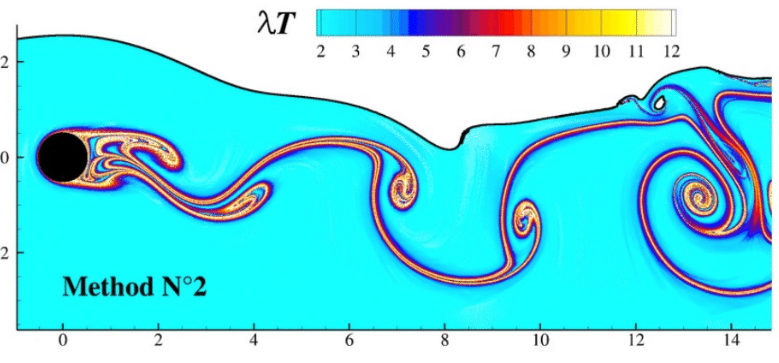
\includegraphics[width=0.55\textwidth]{figures/ch1/15vortex_shedding.png}
	\caption{Left: numerically calculated FTLE field of the ABC flow. Darker colors signify higher FTLE values (Guckenheimer-Holmes Physica D, 2001). Right: Again the FTLE is plotted, for vortex shedding behind a cylinder under a free surface (Sun et. al, 2016).}
	\label{fig:FTLE_flows}
\end{figure}
\end{ex}
\vfill
\section{Dependence on parameters}
We now have the IVP
\begin{align}
	\begin{dcases}
		\dot{ {x}} = f( {x},t, {\mu} ) \\  {x}(t_0) =  {x}_0.
	\end{dcases}
\end{align}
With $ {x} \in \mathbb{R}^{n},\ f\in C^r,\ r\geq 1$, therefore we have a solution $ {x}(t; t_0,  {x}_0,  {\mu} ) \in C^r_{ {x}_0}$.

We now examine how solutions depend $ {\mu } $. This is critical as solutions should be robust to changes or uncertainties in the model.
\begin{ex}[Perturbation Theory]
Given a weakly nonlinear oscillator
\begin{align}
	m \ddot{ x} + c \dot{ x} + k x = \epsilon f(x, \dot{x}, t),\ 0 \leq \epsilon \ll 1,\ x \in \mathbb{R}.
\end{align}
The usual approach is to seek solutions by expanding from the known solution of the linear limit $\epsilon=0$, i.e.
\begin{align}
	x_{\epsilon}(t) = \varphi_0(t) + \epsilon \varphi_1(t) + \epsilon^2 \varphi_2(t) + \ldots + \mathcal{O}(\epsilon^r).
\end{align}
If $x_{\epsilon}(t)$ is in $C^{r}_{\epsilon}$, we have $\varphi_1(t) = \left.\frac{\partial x_\epsilon(t)}{\partial \epsilon}\right \|_{\epsilon =0}$ and $\varphi_2(t) = \left.\frac{\partial^2 x_\epsilon(t)}{\partial \epsilon^2}\right \|_{\epsilon =0}$
\end{ex}

Regularity with respect to the parameter $ {\mu} $ actually follows from regularity with respect to the initial condition $ {x}_0$. We can use the following trick to extend the IVP with a dummy variable $ {\mu} $ 
\begin{align}
	\begin{dcases}
		\dot{ {x}} = f( {x},t,u) \\ \dot{ {\mu}} = 0 \\  {x}(t_0) =  {x}_0 \\  {\mu} (t_0) =  {\mu}_0.
	\end{dcases}
\end{align}
Thus with $ {X}=
\begin{pmatrix}
	 {x} \\  {\mu} 
\end{pmatrix}
\in \mathbb{R}^{n+p}$ and $F( {X}_0) = 
\begin{pmatrix}
	f \\ 0
\end{pmatrix};\  {X}_0 = 
\begin{pmatrix}
	 {x}_0 \\  {\mu} _0
\end{pmatrix}
$. We have the extended IVP
\begin{align*}
	\begin{dcases}
		\dot{ {X}} = F( {X}) \\  {X}(t_0) =  {X}_0.
	\end{dcases} \numberthis \label{eq:ivp_param}
\end{align*}
Applying the previous result on regularity with respect to $ {x}_0$ to \eqref{eq:ivp_param}, we have that $f\in C^{r}_{ {x}, {\mu} }$ implies that $ {X}(t) \in C^{r}_{ {X}_0}$ in turn implying that $ {x}(t; t_0,  {x}_0, \cdot) \in C^{r}_{ {\mu} }$. The solution is as smooth in parameters as the RHS of the dynamical system.

\begin{ex}[Periodic Oscillations of a nonlinear springboard]
\begin{figure}[h!]
	\centering
	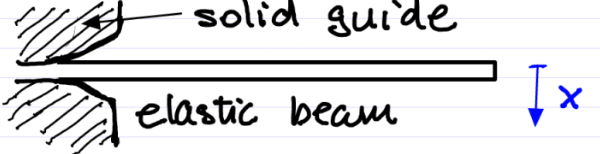
\includegraphics[width=0.6\textwidth]{figures/ch1/16springboard_setup.png}
	\hspace{0.05\textwidth}
	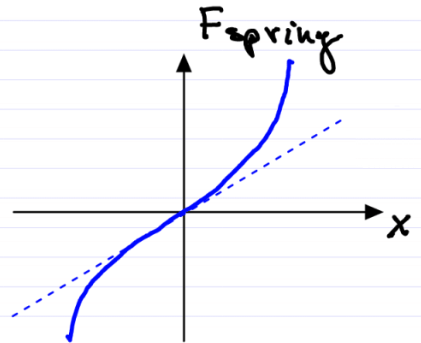
\includegraphics[width=0.3\textwidth]{figures/ch1/17springboard_spring.png}
	\caption{Setup for the nonlinear springboard.}
	\label{fig:nonlin_springboard}
\end{figure}
Given an elastic beam extending from a solid guide, we measure the deflection of this beam with the variable $x$. This system is illustrated in the left panel of Fig. \ref{fig:nonlin_springboard}. By increasing $x$, the effective free length of the beam is shortened, thereby stiffening the spring nonlinearly. The effect of this nonlinearity on the force exerted on the spring is illustrated in the right panel of Fig. \ref{fig:nonlin_springboard}. This setup yields the following equations of motion
\begin{align}
	\begin{dcases}
		\ddot{x} + x + \epsilon x^3 = 0; \quad 0 \leq \epsilon \ll 1 \\
		x(0) = a_0;\quad \dot{x}(0)=0.
	\end{dcases}
\end{align}
So we have weak nonlinearity with no known explicit solution. Although weak, this nonlinearity is still significant, as can be seen in Fig. \ref{fig:effect_nonlin_springboard}. Rewriting this as a first order ODE ($x_1=x;\ x_2=\dot{x}$ ), and note that the RHS is $C^{r}_{ {x}, {\mu} }$, therefore there exists a unique local solution that is also $C^{r}_{ {\mu} }$. Thus the expansion is justified
\begin{align*}
	x_{\epsilon}(t) = \varphi_0(t) + \epsilon \varphi_1(t) + \ldots + \mathcal{O}(\epsilon ^{r}) \numberthis \label{eq:starstar}.	
\end{align*}
We can see that for $\epsilon=0$ we find that $\varphi_0(t) = a_0 \cos(t)$.

Now we look specifically for $T$-periodic solutions, as we would expect such a solution physically, therefore we have
\begin{align}
	\varphi_i(t) = \varphi_i(t+T).
\end{align}
The period $T$ still has to be determined. Plugging this Ansatz to \eqref{eq:starstar} into the IVP to get
\begin{align*}
	&\mathcal{O}(1):\quad \ddot{\varphi}_0 + \varphi_0 &&= 0 \\
	&\mathcal{O}(\epsilon):\quad \ddot{\varphi}_1 + \underbrace{\varphi_1}_{\omega = 1} &&= -\varphi_0^{3} = -a_0^{3}\cos ^{3}(t) = -a_0^{3}\left[ \frac{1}{4} \cos (3t) + \frac{3}{4} \underbrace{ \cos(t)}_{ \textrm{resonance} }\right] \numberthis \label{eq:3star}.
\end{align*}
We can see that \eqref{eq:3star} is a linear oscillator with a forcing coming from the zeroth order solution. Since the zeroth order solution $\varphi_0= a_0 \cos(t)$ already solves the IVP we have the following initial conditions 
\begin{align}
	\varphi_1(0) = 0;\quad \dot{\varphi_1}(t) = 0.
\end{align}
This holds as $\varphi_0 = a_0 \cos(t)$ already solves the IVP. The general solution to this equation is the sum of two terms. We add the general solution of the homogeneous part and a particular solution to the inhomogeneous part. We can write this solution to \eqref{eq:3star} as
\begin{align}
	\varphi_1(t) &= \varphi_1^{ \textrm{hom} }(t) + \varphi_{1}^{ \textrm{part} }(t) \\
		     &= \underbrace{A \cos(t) + B \sin (t)}_{ \textrm{TBD from initial conditions} } + 
		     \underbrace{ C \cos(3t) + D t \cos(t) + Et\sin(t) }_{\textrm{TBD from \eqref{eq:3star}}}.
\end{align}
Observe due to a resonance between the natural frequency of the oscillator and the forcing secular terms, $t \cos(t)$ and $t \sin(t)$ appear. Thus it cannot be periodic, so our Ansatz already fails for $i=1$. We conclude that no solution of this type exists. Our Ansatz was too restrictive and $T$ should depend on $\epsilon$.
\begin{figure}[h!]
	\centering
	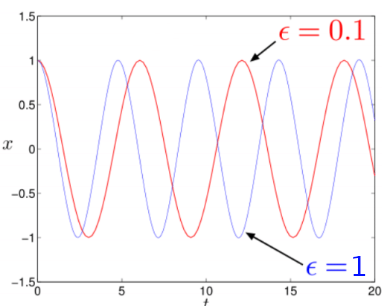
\includegraphics[width=0.3\textwidth]{figures/ch1/18failed_ansatz.png}
	\caption{Numerical integration of $x$ for $a_0=1$ and different values of $\epsilon$.}
	\label{fig:effect_nonlin_springboard}
\end{figure}

\noindent
\textbf{Lindstedt's idea} We should seek a solution of the form
\begin{align}
	x_{\epsilon}(t) = \varphi_0(t;\epsilon) + \epsilon \varphi_1 (t;\epsilon) + \epsilon^2 \varphi_2(t;\epsilon) + \mathcal{O}(\epsilon^3).
\end{align}
Furthermore $\varphi_i$ should be $T_\epsilon$ periodic, i.e. the period should depend on the strength of the  nonlinearity $\epsilon$.
\begin{align}
	\varphi_i(t+T_\epsilon; \epsilon) = \varphi_i(t;\epsilon).
\end{align}
Rewriting the period as
\begin{align}
	T_\epsilon = \frac{2 \pi }{\omega(\epsilon)}; \quad \omega(\epsilon) = 1 + \epsilon \omega_1 + \epsilon^2 \omega_2 + \mathcal{O}(\epsilon^3).
\end{align}
We then rescale time according to $\tau = \omega(\epsilon) t$ to find
\begin{align}
	\frac{d}{d\tau} = \frac{1}{\omega(\epsilon)} \frac{d}{dt} \implies 
	\boxed{[\omega(\epsilon)]^2 x'' + x + \epsilon x^3 = 0.}
\end{align}
Where we have taken $x'$ to represent $\frac{dx}{d\tau}$. Plugging in our new Ansatz into the rescaled ODE yields
\begin{align}
	\left( 1 + 2 \epsilon \omega_1 + \mathcal{O}(\epsilon^2) \right) \left[ \varphi_0'' + \epsilon \varphi'' + \mathcal{O}(\epsilon^2) \right] + \left[ \varphi_0 + \epsilon \varphi_1 + \mathcal{O}(\epsilon^2) \right] + \epsilon \left[\varphi_0^{3} + \mathcal{O}(\epsilon) \right] = 0.
\end{align}
Matching equal powers of $\epsilon$ yields
\begin{align}
	\mathcal{O}(1)&:\ \varphi_0'' + \varphi_0 = 0 \implies \varphi_0(\tau) = a_0 \cos(\tau);\quad \varphi_0(0)=a_0;\quad \dot{\varphi_0}(0) = 0 \\
	\mathcal{O}(\epsilon)&:\ \varphi_1'' + \varphi_1 = - \phi_0^{3} - 2\omega_1 \varphi_{0}'' = 
	\left(2 \omega_1 a_0 - \frac{3}{4}a_0^{3}\right) \underbrace{\cos (\tau)}_{ \textrm{resonance} } - \frac{a_0^{3}}{4} \cos(3 \tau); \\
			     &\phantom{:}\ \varphi_1(0)=0; \quad \dot{\varphi_1}(0) = 0. 
\end{align}
From the first line, we can see the initial conditions are fulfilled. In this step we used that $\dot{\varphi}(t=0) = 0$ if and only if $\omega(\epsilon)\varphi '(0) = 0$. We get the solution
\begin{align}
	\varphi_1(t) = A \cos(\tau) + B \sin(\tau) + C \cos(3\tau) + D\tau \cos(\tau) + E \tau \sin(\tau).
\end{align}
The presence of resonance again excludes periodic solutions, but now we can select $\omega_1$ to eliminate these terms.
\begin{align}
	2\omega_1 a_0 - \frac{3}{4} a_0 ^{3} = 0 \implies \boxed{\omega_1 = \frac{3}{8}a_0^{2}.}
\end{align}
This successfully eliminates the resonance and determines the missing frequency term at $\mathcal{O}(\epsilon)$. Thus we find
\begin{align}
	x_\epsilon(\tau) = a_0 \cos(\tau) - \frac{\epsilon}{32}a_0^{3}\left( \cos(\tau) - \cos (3\tau) \right) + \mathcal{O}(\epsilon^2).
\end{align}
In the original time scaling this is
\begin{align}
	x_\epsilon (t) = a_0 \cos (\omega t) - \frac{\epsilon}{32} a_0^3 \left( \cos(\omega t) - \cos(3\omega t)\right) + \mathcal{O}(\epsilon^2); \quad \omega = 1+ \frac{3}{8}\epsilon a_0^2 + \mathcal{O}(\epsilon^2).	
\end{align}
This procedure can be continued to higher order terms, where we select $\omega_2$ so that the $\mathcal{O}(\epsilon^2)$ terms cancel.
\begin{figure}[h!]
	\centering
	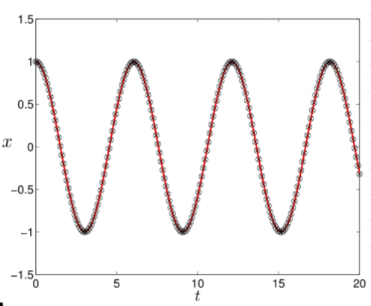
\includegraphics[width=0.45\textwidth]{figures/ch1/19approximation_accuracy.png}
	\caption{Approximation (dots) vs analytic solution (solid line) of $x$ on the time interval $[0,20]$.}
\end{figure}

\end{ex}
